 \documentclass[10pt, table, dvipsnames,xcdraw,handout]{beamer}
\usetheme[progressbar=frametitle]{metropolis}
\usepackage{appendixnumberbeamer}
\usetikzlibrary{arrows.meta, positioning, quotes}
\usepackage[shortlabels]{enumitem}
\usepackage{xcolor}
\usepackage{mathtools}


\usepackage{cancel}

\newcommand\hcancel[2][black]{\setbox0=\hbox{$#2$}%
\rlap{\raisebox{.45\ht0}{\textcolor{#1}{\rule{\wd0}{1pt}}}}#2} 


\usepackage{booktabs}
\usepackage[scale=2]{ccicons}

\usepackage{pgfplots}
\usepgfplotslibrary{dateplot}

\usepackage{xspace}
\newcommand{\themename}{\textbf{\textsc{metropolis}}\xspace}
\newcommand{\cb}{\cellcolor{blue!25}}


% Notation:
\newcommand{\cT}{\ensuremath{\mathcal{T}}}
\newcommand{\cD}{\ensuremath{\mathcal{D}}}
\newcommand{\cX}{\ensuremath{\mathcal{X}}}
\newcommand{\cY}{\ensuremath{\mathcal{Y}}}
\newcommand{\cZ}{\ensuremath{\mathcal{Z}}}
\newcommand{\cH}{\ensuremath{\mathcal{H}}}
\newcommand{\cG}{\ensuremath{\mathcal{G}}}

\newcommand{\bR}{\ensuremath{\mathbb{R}}}
\newcommand{\bN}{\ensuremath{\mathbb{N}}}
\newcommand{\bP}{\ensuremath{\mathbb{P}}}
\newcommand{\bT}{\ensuremath{\mathbb{T}}}
\newcommand{\bL}{\ensuremath{\mathbb{L}}}

\newcommand{\bfX}{\ensuremath{\mathbf{X}}}
\newcommand{\bfY}{\ensuremath{\mathbf{Y}}}
\newcommand{\bfy}{\ensuremath{\mathbf{y}}}

\def\layersep{2.5cm}

% Tikz seys
\tikzset{cross/.style={cross out, draw, 
         minimum size=2*(#1-\pgflinewidth), 
         inner sep=0pt, outer sep=0pt}}

\title{Machine Learning I}
\subtitle{Lecture 11: Training Deep Networks}
% \date{\today}
\date{}
\author{Nathaniel Bade}
\institute{Northeastern University Department of Mathematics}
% \titlegraphic{\hfill\includegraphics[height=1.5cm]{logo.pdf}}

\begin{document}

\maketitle

\begin{frame}{Table of contents}
  \setbeamertemplate{section in toc}[sections numbered]
  \tableofcontents[hideallsubsections]
\end{frame}


%%%%%%%%%%%%%% Slidshow Start %%%%%%%%%%%%%% 



\section{Vanishing Gradients and Activation Functions}
\begin{frame}[fragile]{Genre of Artificial Neural Networks}
Training deep neural networks is \textbf{hard}. Even with back-propagation is easy to propose networks that are practically impossible to train. In addition, some problems may require very large or very deep networks.

Some common problems with training:

\begin{itemize}
\item[] Vanishing and exploding gradients.\pause
\item[] Not enough training data for the network size, or not enough labeled data.\pause
\item[] Training may slow.\pause
\item[] Models with too many parameters may severely overfit.
\end{itemize}

There are a number of schemes to tackle each of these problems, but at the end of the day knowing the solutions and your data is vital in helping you choose how to overcome them. 
\end{frame}




\begin{frame}[fragile]{Vanishing Gradients}
\begin{minipage}[t][0.5\textheight][t]{\textwidth}\centering
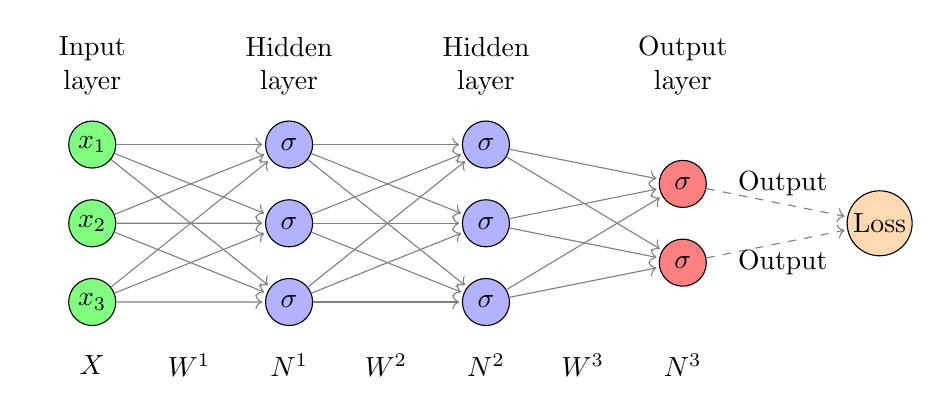
\begin{tikzpicture}[shorten >=1pt,->,draw=black!50, node distance=\layersep]
%https://tex.stackexchange.com/questions/96846/how-to-place-label-in-middle-of-line-above-and-below-with-tikz
    \tikzstyle{every pin edge}=[<-,shorten <=1pt]
    \tikzstyle{neuron}=[circle,fill=black!25,minimum size=17pt,inner sep=0pt, draw=black]
    \tikzstyle{input neuron}=[neuron, fill=green!50];
    \tikzstyle{output neuron}=[neuron, fill=red!50];
    \tikzstyle{hidden neuron}=[neuron, fill=blue!30];
    \tikzstyle{loss neuron}=[neuron, fill=orange!30];
    \tikzstyle{annot} = [text width=4em, text centered]

    % Draw the input layer nodes
    \foreach \name / \y in {1,...,3}
    % This is the same as writing \foreach \name / \y in {1/1,2/2,3/3,4/4}
        \node[input neuron] (I-\name) at (0,-\y) {$x_\y$};

    % Draw the hidden layer nodes
    \foreach \name / \y in {1,...,3}
        \path[yshift=0cm]
            node[hidden neuron] (H1-\name) at (\layersep,-\y cm) {$\, \sigma\, $};

    % Draw the hidden layer nodes
    \foreach \name / \y in {1,...,3}
        \path[yshift=0cm]
            node[hidden neuron] (H2-\name) at (\layersep + \layersep,-\y cm) {$\, \sigma\, $};


    % Draw the output layer node
    \foreach \name / \y in {1,...,2}
    		\node[output neuron] (O-\y) at (\layersep + \layersep + \layersep,-\y cm-.5cm) {$\,\sigma\,$};
    		
    		
    		
    		\node[loss neuron] (L) at (\layersep +\layersep + \layersep + \layersep,-2 cm) {$\,$Loss$\,$};

    % Connect every node in the input layer with every node in the
    % hidden layer.
    \foreach \source in {1,...,3}
        \foreach \dest in {1,...,3}
            \draw (I-\source) --  (H1-\dest);

    % Connect every node in the input layer with every node in the
    % hidden layer.
    \foreach \source in {1,...,3}
        \foreach \dest in {1,...,3}
            \draw (H1-\source) --  (H2-\dest);


    % Connect every node in the hidden layer with the output layer
    \foreach \source in {1,...,3}
		\foreach \dest in {1,...,2}
        		\path (H2-\source) edge (O-\dest);
        		
		\foreach \source in {1,...,2}
        		\path[dashed] (O-\source) edge (L);

    % Annotate the layers
    \node[annot, right of=O-1,xshift=-35] {Output};
    \node[annot, right of=O-2,xshift=-35] {Output};
    \node[annot,above of=H1-1, node distance=1cm] (hl) {Hidden layer};
    \node[annot,left of=hl] {Input layer};
    \node[annot,right of=hl] (hl2) {Hidden layer};
    \node[annot,right of=hl2] {Output layer};
    
    \node[annot,below of=H1-3, node distance=.8cm] (hb) {$N^1$};
    \node[annot,left of=hb] {$X$};
    \node[annot,right of=hb] (hb2) {$N^2$};
    \node[annot,right of=hb2] {$N^3$};
    \node[annot,left of=hb,xshift=35] {$W^1$};
    \node[annot,xshift=35] at (hb) {$W^2$};
    \node[annot,xshift=35]  at (hb2) {$W^3$};
\end{tikzpicture}
  \end{minipage}
  \vfill
\begin{minipage}[t][0.5\textheight][t]{\textwidth}
Lets consider a deep perceptron network with $N$ hidden layers. For a given input $X$, the values at each layer are computed by
$$
N^{i} = \sigma(W^{i}N^{i-1} + b^{i})
$$ 
The loss function finally is some non-negative function of the outputs. 
\end{minipage}
\end{frame}






\begin{frame}[fragile]{Vanishing Gradients}
\begin{minipage}[t][0.5\textheight][t]{\textwidth}\centering
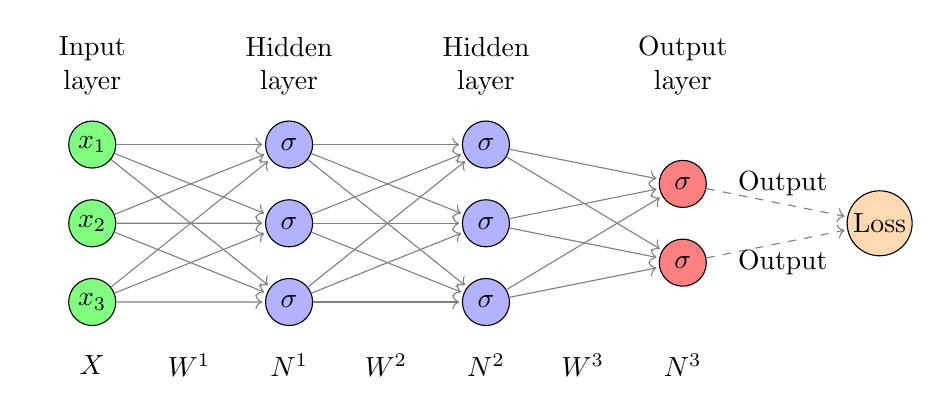
\begin{tikzpicture}[shorten >=1pt,->,draw=black!50, node distance=\layersep]
%https://tex.stackexchange.com/questions/96846/how-to-place-label-in-middle-of-line-above-and-below-with-tikz
    \tikzstyle{every pin edge}=[<-,shorten <=1pt]
    \tikzstyle{neuron}=[circle,fill=black!25,minimum size=17pt,inner sep=0pt, draw=black]
    \tikzstyle{input neuron}=[neuron, fill=green!50];
    \tikzstyle{output neuron}=[neuron, fill=red!50];
    \tikzstyle{hidden neuron}=[neuron, fill=blue!30];
    \tikzstyle{loss neuron}=[neuron, fill=orange!30];
    \tikzstyle{annot} = [text width=4em, text centered]

    % Draw the input layer nodes
    \foreach \name / \y in {1,...,3}
    % This is the same as writing \foreach \name / \y in {1/1,2/2,3/3,4/4}
        \node[input neuron] (I-\name) at (0,-\y) {$x_\y$};

    % Draw the hidden layer nodes
    \foreach \name / \y in {1,...,3}
        \path[yshift=0cm]
            node[hidden neuron] (H1-\name) at (\layersep,-\y cm) {$\, \sigma\, $};

    % Draw the hidden layer nodes
    \foreach \name / \y in {1,...,3}
        \path[yshift=0cm]
            node[hidden neuron] (H2-\name) at (\layersep + \layersep,-\y cm) {$\, \sigma\, $};


    % Draw the output layer node
    \foreach \name / \y in {1,...,2}
    		\node[output neuron] (O-\y) at (\layersep + \layersep + \layersep,-\y cm-.5cm) {$\,\sigma\,$};
    		
    		
    		
    		\node[loss neuron] (L) at (\layersep +\layersep + \layersep + \layersep,-2 cm) {$\,$Loss$\,$};

    % Connect every node in the input layer with every node in the
    % hidden layer.
    \foreach \source in {1,...,3}
        \foreach \dest in {1,...,3}
            \draw (I-\source) --  (H1-\dest);

    % Connect every node in the input layer with every node in the
    % hidden layer.
    \foreach \source in {1,...,3}
        \foreach \dest in {1,...,3}
            \draw (H1-\source) --  (H2-\dest);


    % Connect every node in the hidden layer with the output layer
    \foreach \source in {1,...,3}
		\foreach \dest in {1,...,2}
        		\path (H2-\source) edge (O-\dest);
        		
		\foreach \source in {1,...,2}
        		\path[dashed] (O-\source) edge (L);

    % Annotate the layers
    \node[annot, right of=O-1,xshift=-35] {Output};
    \node[annot, right of=O-2,xshift=-35] {Output};
    \node[annot,above of=H1-1, node distance=1cm] (hl) {Hidden layer};
    \node[annot,left of=hl] {Input layer};
    \node[annot,right of=hl] (hl2) {Hidden layer};
    \node[annot,right of=hl2] {Output layer};
    
    \node[annot,below of=H1-3, node distance=.8cm] (hb) {$N^1$};
    \node[annot,left of=hb] {$X$};
    \node[annot,right of=hb] (hb2) {$N^2$};
    \node[annot,right of=hb2] {$N^3$};
    \node[annot,left of=hb,xshift=35] {$W^1$};
    \node[annot,xshift=35] at (hb) {$W^2$};
    \node[annot,xshift=35]  at (hb2) {$W^3$};
\end{tikzpicture}
  \end{minipage}
  \vfill
\begin{minipage}[t][0.5\textheight][t]{\textwidth}
Back propegation computes the gradient of the weights $W^k$ of the $k$'th layer via the chain rule
$$
\frac{\partial \, \text{Loss}}{\partial W^{k} } 
=
\frac{\partial \, \text{Loss}}{\partial W^{K} } 
\frac{\partial  W^{K}}{\partial W^{K-1} } 
\ldots
\frac{\partial  W^{k+1}}{\partial W^{k} } 
$$
This lead to the following issue: If the gradients of the final weights vanish, all previous gradients will as well.
\end{minipage}
\end{frame}







\begin{frame}[fragile]{Vanishing Gradients}
This \textbf{vanishing gradient problem} was observed empirically in the last century, and is one of the reasons deep neural networks we abandoned in the early 2000's. However, a 2010 paper by \href{http://proceedings.mlr.press/v9/glorot10a/glorot10a.pdf}{Glorot and Benigo} performed some explorations on the training of deep networks and made some progress on solving them

Glorot and Benigo noted a few things about training networks: First, they showed that using the at-the-time standard initialization of a uniform distribution for the weights $W^i_{ij} = U(-n_{i-1}^{-\frac12},n_{i-1}^{-\frac12})$ along with the sigmoid activation function resulted in a strict decrease in the weight variance for layers farther from the output. 

\end{frame}




\begin{frame}[fragile]{Vanishing Gradients}
  \begin{minipage}[t][0.5\textheight][t]{\textwidth}
	\centering \includegraphics[width=0.8\textwidth]{L11VanishingGrad1.png} 
  \end{minipage}
  \vfill
\begin{minipage}[t][0.5\textheight][t]{\textwidth}
The diagram above shows the back-propagated gradients for a 5 layer networks with 1000 nodes per layer using sigmoid activation and the standard initialization from the last last slide.  Practically, this means that the earlier layers take much longer to train, as their gradients are much smaller.
\end{minipage}
\end{frame}



\begin{frame}[fragile]{Vanishing Gradients}
  \begin{minipage}[t][0.5\textheight][t]{\textwidth}
	\centering \includegraphics[width=0.8\textwidth]{L11VanishingGrad2.png} 
  \end{minipage}
  \vfill
\begin{minipage}[t][0.5\textheight][t]{\textwidth}
In addition, they showed that as the data passes through the network, the activation values $N^i$ of the last layer are rapidly driven to 0. The chary above shows the mean and standard deviation of the output of each activation layer.
\end{minipage}
\end{frame}



\begin{frame}[fragile]{Vanishing Gradients}
  \begin{minipage}[t][0.5\textheight][t]{\textwidth}
	\centering \includegraphics[width=0.8\textwidth]{L11VanishingGrad2.png} 
  \end{minipage}
  \vfill
\begin{minipage}[t][0.5\textheight][t]{\textwidth}
We see empirically that the activations of the final hidden layer $N^K$ rapidly drop to 0 and as a result training nearly stops for the first 100 epochs. However, at epoch 100, $N^K$ activations slowly desaturate, allowing training to propagate down. 
\end{minipage}
\end{frame}





\begin{frame}[fragile]{Vanishing Gradients}
  \begin{minipage}[t][0.5\textheight][t]{\textwidth}
	\centering \includegraphics[width=0.8\textwidth]{L11VanishingGrad3.png} 
  \end{minipage}
  \vfill
\begin{minipage}[t][0.5\textheight][t]{\textwidth}
Finally, their experiments showed that when using tanh activation functions, the variance of the activations $N^k$ decreases as we move forward through the network. They conclude again this this is another face of the the signal ``dying out'' as the data moves through a deep neural network. 
\end{minipage}
\end{frame}


\begin{frame}[fragile]{Vanishing Gradients}
Glorot and Bengio propose that to alleviate these issues we need to ensure that information is flowing correctly backwards and forwards at each step of the network. They propose that the correction is to fix the network so the outputs of each layer have equal variance, and that the gradients flowing back through each layer have equal variance. 

Glorot and Bengio perform an explicit computation of the variance loss, finding a factor of 1/3n between layers both with $n$ nodes. They proposed that by treating $n = n_{avg} = \frac{n_i + n_{i+1}}2$ as the average number of nodes in the two layer and using a uniform initialization of 
$$
W^i \sim U\left( -\sqrt{\frac{6}{n_i + n_{i+1}}}, \sqrt{\frac{3}{n_{avg}}}  \right)\,,
$$
that the variance would be fixed. Their paper provided a nice computation, as well as empirical verification of the effectiveness of this normalization. This is known as \textbf{Glorot Initialization}.
\end{frame}



\begin{frame}[fragile]{Vanishing Gradients}
Glorot initialization can drastically speed up deep learning. It was later extended to the following normal distribution formula
$$
W^i \sim \mathcal{N}\left(0,1/ n_{avg}\right)\,,
$$
and subsequent authors have repeated their analysis for other activation functions

\begin{table}[]
\begin{tabular}{lll}
\multicolumn{1}{l|}{Initialization} & Activation Function           & Normal Variance $\sigma^2$ \\ \hline
\multicolumn{1}{l|}{Glorot}         & None, tanh, logistic, softmax & $1/n_{ave}$                \\
He                                  & ReLU variants                 & $2/n_{in}$                 \\
LeCun                               & SELU                          & $1/n_{in}$                
\end{tabular}
\end{table}

Here, $n_{in}$ is the number of nodes in the previous layer. Keras uses Glorot by default, but can be changed to use any other initialization.


\end{frame}




\begin{frame}[fragile]{Vanishing Gradients}
Before Glorot and Bengio's paper the role of the activation functions hadn't been considered deeply, and were either seen as an arbitrary normalization that the weights would compensate for, or as coming ``philosophically'' from the sigmoid activation in biological neurons. After the spot light was put on the activation functions, it was discovered that often other functions work much better.
\end{frame}


\begin{frame}[fragile]{Activation Functions}
  \begin{minipage}[t][0.5\textheight][t]{\textwidth}
	\centering \includegraphics[height=0.5\textheight]{L11Activations1.png} 
  \end{minipage}
  \vfill
\begin{minipage}[t][0.5\textheight][t]{\textwidth}
The ReLU function has been shown to work very well across a wide variety of applications, since it is both simple to compute and does not saturate for large values. However, it suffers from the \textbf{dying ReLUs} problem, where neurons stop outputting anything except 0. This happens if the incoming weights get tweeked so that the input is always negative. For large learning rates, its not uncommon to find half of the neurons dead.
\end{minipage}
\end{frame}


\begin{frame}[fragile]{Activation Functions}
  \begin{minipage}[t][0.5\textheight][t]{\textwidth}
	\centering \includegraphics[height=0.5\textheight]{L11Activations2.png} 
  \end{minipage}
  \vfill
\begin{minipage}[t][0.5\textheight][t]{\textwidth}
One fix is to use the \textbf{Leaky ReLU} function
$$
\textbf{Leaky ReLU}(z) = \text{max}(\alpha z,z)\,, \alpha<1.\,.
$$
The hyperparameter $\alpha$ is usually set to .01, and the small slope ensures the activations never die.
\end{minipage}
\end{frame}



\begin{frame}[fragile]{Activation Functions}
  \begin{minipage}[t][0.5\textheight][t]{\textwidth}
	\centering \includegraphics[height=0.5\textheight]{L11Activations2.png} 
  \end{minipage}
  \vfill
\begin{minipage}[t][0.5\textheight][t]{\textwidth}
Many ReLU's variants have been tested over the years and leaky ReLU's is consistently one of the top performers. Other ReLU's function include \textbf{randomized ReLUs} where $\alpha$ is picked randomly on each training run and \textbf{parametric ReLUs}, where $\alpha$ is a fittable parameter.  The latter has been shown to outperform ReLU on large image datasets, but to overfit on small ones. 
\end{minipage}
\end{frame}



\begin{frame}[fragile]{Activation Functions}
  \begin{minipage}[t][0.5\textheight][t]{\textwidth}
	\centering \includegraphics[height=0.5\textheight]{L11Activations3.png} 
  \end{minipage}
  \vfill
\begin{minipage}[t][0.5\textheight][t]{\textwidth}
Finally, the exponential linear unit \textbf{ELU} is
$$
\textbf{ELU}(z) = \begin{cases}
\alpha (e^z - 1)&\text{for} z<0\,,
\\
z&\text{for} z>0\,.
\end{cases}
$$
Introduced in 2015, ELU's outperformed all ReLU's variants in a large series of classification tasks, providing better accuracy while lowering the number of training steps. 
\end{minipage}
\end{frame}




\begin{frame}[fragile]{Activation Functions}
  \begin{minipage}[t][0.5\textheight][t]{\textwidth}
	\centering \includegraphics[height=0.5\textheight]{L11Activations3.png} 
  \end{minipage}
  \vfill
\begin{minipage}[t][0.5\textheight][t]{\textwidth}
The ELU is negative when $z<0$, and has nonzero gradient everywhere, avoiding the dead neuron problem. It is also smooth for $\alpha=1$, which can help to avoid a wildly bouncing gradient for $z\approx 0$. The only drawback is in the computation of the exponential, meaning that at use time the network will be slower than a ReLU network.
\end{minipage}
\end{frame}






\begin{frame}[fragile]{Activation Functions}
  \begin{minipage}[t][0.5\textheight][t]{\textwidth}
	\centering \includegraphics[height=0.5\textheight]{L11Activations4.png} 
  \end{minipage}
  \vfill
\begin{minipage}[t][0.5\textheight][t]{\textwidth}
Finally, in 2017 Klambauer et al introduced the \text{Scaled ELU}
$$
\textbf{SELU}(z) = \lambda\begin{cases}
\alpha (e^z - 1)&\text{for} z<0\,,
\\
z&\text{for} z>0\,.
\end{cases}
$$
The authors showed that a deep perceptron network built exclusively of SELU units is \emph{self normalizing}, in that the output of each layer will tend towards a mean of 0 and std of 1. 
\end{minipage}
\end{frame}



\begin{frame}[fragile]{Activation Functions}
  \begin{minipage}[t][0.5\textheight][t]{\textwidth}
	\centering \includegraphics[height=0.5\textheight]{L11Activations4.png} 
  \end{minipage}
  \vfill
\begin{minipage}[t][0.5\textheight][t]{\textwidth}
However, the SELU has a few requirements:

\begin{itemize}
\item The data must be normalized to be between 0 and 1.
\item The weights must be normalized to the LeCune Normalization $\mathcal{N}(0,\frac{1}{n_{in}})$.
\item The architecture must be sequential dense layers. 
\end{itemize}
\end{minipage}
\end{frame}


\begin{frame}[fragile]{Activation Functions}
  \begin{minipage}[t][0.5\textheight][t]{\textwidth}
	\centering \includegraphics[height=0.5\textheight]{L11Activations4.png} 
  \end{minipage}
  \vfill
\begin{minipage}[t][0.5\textheight][t]{\textwidth}
So which should you use? The current wisdom is 
$$
\text{SELU}>\text{ELU}>\text{Leaky ReLU}>\text{ReLU}>\sigma,\,\tanh, \text{etc.} 
$$
For example, if you cannot use SELU (for example in a CNN) use a ELU, or care deeply about runtime speed, you can use Leaky ReLU instead. 
\end{minipage}
\end{frame}


\section{Batch Normalization and Gradient Clipping}



\begin{frame}[fragile]{Activation Functions}
Proper normalization can drastically reduce the vanishing/exploding gradient problem out the outset but it can come back during training. The are several methods to tackle this problem, including \textbf{batch normalization} and \textbf{gradient clipping}. 

For \textbf{batch normalization}, we add an operation in the model before each layer that trieds to learn the optimal scale and offset for the data. The layer zero-centers and scales each input with respect to a given mini-batch, and then shifts and scales the input via two trainable parameters. 
\end{frame}



\begin{frame}[fragile]{Batch Normalization}
Concretely, for each minibatch of $M$ input data points $x_i$, $i=1,\ldots M$, the batch normalization algorithm computes the batch mean and variance
$$
\hat{\mu} = \frac{1}{M}\sum_{i=1}^M x_i\,,\hspace{3em} \hat{\sigma}^2 = \frac{1}{M}\sum_{i=1}^M (x_i - \hat{\mu})^2\,,
$$
normalizes the input data ($\epsilon \approx 10^{-5}$ avoids divide by 0 errors)
$$
\tilde{x}_i = \frac{x_i - \hat{\mu}}{\sqrt{\hat{\sigma}^2 + \epsilon}}\,,
$$
and then scales and shifts the data component-wise
$$
\hat{x}_i =  D_\gamma \tilde{x}_i + \beta\,.
$$
Here, $D_\gamma $ is a diagonal scaling matrix with entries $D_{jj} = \gamma_j$. The vectors $\gamma$ and $\beta$ are trainable parameters that select the optimal scale of the data. 
\end{frame}




\begin{frame}[fragile]{Batch Normalization}
In their 2015 paper on the introducing batch normalization, Ioffe and Szegedy demonstrated that batch normalization improved all tested deep neural networks. In fact,  they managed to reduce the vanishing gradient problem so much that saturating activation functions like $\sigma$ and tanh could be efficiently used. In addition the weights were more stable during learning and so much larger learning rates could be used. \pause

There are two problems with batch normalization however, both of which come at runtime: First, the extra layer lead to a run time disadvantage. That said, after training the batch normalization layer can be fused back into the previous weight layer by an overall rescaling. \pause

Second, it is not clear how to send a single new sample through the network, since the batch normalization layer relies on minibatch data. This is usually solved by computing a moving average over all training batches of the fit mean $\hat{\mu}$ and variance $\hat{\sigma}^2$ at training time, but this of course might have trouble accounting for new data. 

\end{frame}




\begin{frame}[fragile]{Batch Normalization and Gradient Clipping}
Batch Normalization is the current state of the art for neural networks, to the degree that it's often just assumed and omitted from network diagrams. It's easy to implement using Keras's inbuilt batch normalization layers.\pause

Gradient clipping is another standard technique for solving the gradient explosion problem. The idea behind gradient clipping is straight forward: At optimization time, set the optimize to trim any gradient components that are above some value $\alpha$, where usually $\alpha = 1$. In practice this approach works well and can be computed per-weight, although you are potentially changing the gradient direction. \pause

A second option is to scale the gradient to a constant value. In practice, this will allow one large direction to dominate the training, but still can work well. If you're network is not training and you notice your weights are exploding it is worth trying both. 
\end{frame}



\section{Faster Optimizers}



\begin{frame}[fragile]{Optimizers}
In the last few sections we discussed several ways in speeding up network training by tuning the activation functions and the initial conditions to ensure we start in a trainable place and by normalizing the layer inputs and gradients to ensure we stay there. We now want to turn our attention to the (stochastic) gradient decent step. 

There are several ways we can improve gradient decent, mostly by being more responsive to the local geometry of the loss function and the previous steps we taken. In the following sections, we will describe Momentum Optimzation, AdaGrad, and the Adam optimizer and discuss the advantages they have over vanilla SGD.
\end{frame}




\begin{frame}[fragile]{Momentum Optimization}
  \begin{minipage}[t][0.5\textheight][t]{\textwidth}
	\centering \includegraphics[height=0.5\textheight]{L11MomentumDecent.png} 
  \end{minipage}
  \vfill
\begin{minipage}[t][0.5\textheight][t]{\textwidth}
Imagine rolling a bowling ball down a slope. As the ball picks up momentum it moves faster and faster towards the local minimum. As a contrast, gradient decent is like walking down a wide stare, stopping at each step and considering what to do next. 
\end{minipage}
\end{frame}



\begin{frame}[fragile]{Momentum Optimization}
  \begin{minipage}[t][0.5\textheight][t]{\textwidth}
	\centering \includegraphics[height=0.5\textheight]{L11MomentumDecent.png} 
  \end{minipage}
  \vfill
\begin{minipage}[t][0.5\textheight][t]{\textwidth}
For a loss function $L$, and a network with weights $W$, gradient decent proceeds by computing the $i+1$'st step by
$$
W^{(i+1)} = W^{(i)} - \eta \nabla_W L\,.
$$
When $\nabla_W L$ is small (say, at the bottom of a shallow basin in our bowling ball example), training will proceed painfully slowly. 
\end{minipage}
\end{frame}



\begin{frame}[fragile]{Momentum Optimization}
  \begin{minipage}[t][0.5\textheight][t]{\textwidth}
	\centering \includegraphics[height=0.5\textheight]{L11MomentumDecent.png} 
  \end{minipage}
  \vfill
\begin{minipage}[t][0.5\textheight][t]{\textwidth}
In momentum optimization, the parameters are updated in the direction of the momentum vector $m$. At each iteration, we use the gradient to update the momentum
$$
m^{(i+1)}= \alpha m^{(i)} -\eta \nabla_{W} L\,,\hspace{3em} W^{(i+1)} = W^{(i)}+m^{(i+1)}\,,
$$
where $\alpha$ is a new hyperparameter that keeps $m$ from getting too large. 
\end{minipage}
\end{frame}




\begin{frame}[fragile]{Momentum Optimization}
  \begin{minipage}[t][0.5\textheight][t]{\textwidth}
	\centering \includegraphics[height=0.5\textheight]{L11MomentumDecent2.png} 
  \end{minipage}
  \vfill
\begin{minipage}[t][0.5\textheight][t]{\textwidth}
If the gradient $ \nabla_{W} L$ is constant, than the momentum optimizer's terminal velocity is given by the geometric series
$$
\lim_{i\to \infty} m^{(i)} = -\sum_{n=0}^\infty \alpha^n \eta  \nabla_{W} L = \frac{1}{1-\alpha}  \eta \nabla_{W} L\,,
$$
so for $\alpha \approx 1$ the ``terminal velocity'' of the momentum optimize is much faster than the gradient decent optimizer. 
\end{minipage}
\end{frame}





\begin{frame}[fragile]{Momentum Optimization}
  \begin{minipage}[t][0.5\textheight][t]{\textwidth}
	\centering \includegraphics[height=0.5\textheight]{L11MomentumDecent2.png} 
  \end{minipage}
  \vfill
\begin{minipage}[t][0.5\textheight][t]{\textwidth}
If the gradient $ \nabla_{W} L$ is constant, than the momentum optimizer's terminal velocity is given by the geometric series
$$
\lim_{i\to \infty} m^{(i)} = -\sum_{n=0}^\infty \alpha^n \eta  \nabla_{W} L = \frac{1}{1-\alpha}  \eta \nabla_{W} L\,,
$$
so for $\alpha \approx 1$ the ``terminal velocity'' of the momentum optimize is much faster than the gradient decent optimizer. 
\end{minipage}
\end{frame}





\begin{frame}[fragile]{Nesterov Accelerated Gradient}
On small addition to momentum gradient decent was made in 1983 by Nesterov. Instead of measuring the gradient of the cost function at $W^{(i)}$, we should measure it a little bit ahead in the momentum direction $W^{(i)} + m^{(i)}$. The equations become
$$
m^{(i+1)}= \alpha m^{(i)} -\eta \nabla_{W} L(W^{(i)} + m^{(i)})\,,\hspace{3em} W^{(i+1)} = W^{(i)}+m^{(i+1)}\,.
$$

This is unsurprising, there is no reason to think that the gradient is the best update to the moment. The idea here is to try to correct the momentum by looking ahead a down the road. If the local geometry is the same a little bit ahead than the correction does no harm. But if the local geometry changes, we get a head start making the turn. 
\end{frame}




\begin{frame}[fragile]{Nesterov Accelerated Gradient}
  \begin{minipage}[t][0.5\textheight][t]{\textwidth}
	\centering \includegraphics[height=0.5\textheight]{L11Geron1.png} 
  \end{minipage}
  \vfill
\begin{minipage}[t][0.5\textheight][t]{\textwidth}
In the figure above (Geron, 11-6) the regular momentum update would not take into account the fact the $m + \nabla L$ takes the function up the far the wall. Evaluating the gradient at $W^{(i)}+m^{(i)}$ give the correct ``best way forward'' for the next update step. 
\end{minipage}
\end{frame}





\begin{frame}[fragile]{AdaGrad}
  \begin{minipage}[t][0.5\textheight][t]{\textwidth}
	\centering \includegraphics[height=0.5\textheight]{L11AdaGrad.png} 
  \end{minipage}
  \vfill
\begin{minipage}[t][0.5\textheight][t]{\textwidth}
Lets consider another potential problem: Assume the loss function takes the shape of an elongated bowl in one direction near the minimum. The gradient then wont point towards the minimum, instead making a series of over corrections while we slowly walk along the less steep direction towards to the origin. 
\end{minipage}

\end{frame}



\begin{frame}[fragile]{AdaGrad}
  \begin{minipage}[t][0.5\textheight][t]{\textwidth}
	\centering \includegraphics[height=0.5\textheight]{L11AdaGrad.png} 
  \end{minipage}
  \vfill
\begin{minipage}[t][0.5\textheight][t]{\textwidth}
Overshooting the learning rate is a huge problem here: If we set the learning rate high enough that we make substantial progress in the shallow direction we will almost certainly bounce away from the minimum in the steeper direction. 
\end{minipage}
\end{frame}


\begin{frame}[fragile]{AdaGrad}
The \textbf{adaptive subgradient methods} or \textbf{AdaGrad} solves this problem by scaling the update vector to avoid letting one direction dominate. Let $s$ be the scale vector. At each iterative step, we update $s$ by
$$
s_j^{(i+1)} = s_j^{(i)} + (\nabla_{W} L) _j^2\,,\hspace{3em} j=1,\ldots, p\,.
$$\pause
Then, we define a scaled gradient componentwise
$$
(\hat{\nabla_{W} L})_j = (\nabla_{W} L)_j/\sqrt{s_j^{(i+1)}+\epsilon} \,,
$$
Where again $\epsilon$ is a small constant to avoid divide by 0 errors.  \pause The decent step becomes the scaled decent step
$$
W^{(i+1)} = W^{(i)} - \eta \hat{\nabla_{W} L}\,.
$$\pause

AdaGrad performs well for simple quadratic problems, but it often stops early for more complicated optimizations like neural networks. 
\end{frame}



\begin{frame}[fragile]{RMSProp}
One of the reasons AdaGrad slows so rapidly is that it's hard for a weight to recover from having a large gradient earlier on in the training cycle.  \textbf{RMSProp} (Root Mean Square Propagation) provides a fix to AdaGrads slowing by only remembering the most recent gradients. It does this by introducing an exponential decay step: The scaling vector now depends on a hyperparamter $\alpha$
$$
s_j ^{(i+1)}= \alpha s_j^{(i+1)} + (1-\alpha) (\nabla_{W} L) _j^2\,,\hspace{3em} j=1,\ldots, p\,.
$$\pause
This fix provides a huge improvement the training efficiency over the standard AdaGrade algorithm, and makes it feasible to train neural networks. 

\end{frame}



\begin{frame}[fragile]{Adam Optimizer}
Finally, the \textbf{Adam optimizer} (adaptive momentum estimate) combines both momentum optimization and the adaptive scale fixing of RMSProp: The momentum are scaling vectors are updates as for Momentum and RMSProp
\begin{align*}
m^{(i+1)} &= \alpha_1 m^{(i)} + (1-\alpha_1) \nabla_{W} L\,,
\\
s_j^{(i+1)} &= \alpha_2 s_j^{(i+1)} + (1-\alpha) (\nabla_{W} L) _j^2\,,j=1,\ldots, p\,.
\end{align*}\pause
The biases are then given a step dependent update to help force them away from their initial value of 0:
\begin{align*}
\hat{m}^{(i+1)} = \frac{{m}^{(i+1)}}{1-\alpha^i_1}\,,\hspace{1em}
\hat{s}^{(i+1)} = \frac{{s}^{(i+1)}}{1-\alpha^i_2}\,.
\end{align*}\pause
Finally, the update step is a scaled momentum update:
\begin{align*}
(\hat{\nabla_{W} L})_j &= \hat{m}^{(i+1)}_j/\sqrt{s_j^{(i+1)}+\epsilon} \,,
\\
W^{(i+1)} &= W^{(i)} - \eta \hat{\nabla_{W} L}\,.
\end{align*}

\end{frame}



\begin{frame}[fragile]{Adam Optimizer}
Two notes about Adam: First, since $\alpha_k<1$, the second step scaling 
\begin{align*}
\hat{m}^{(i+1)} = \frac{{m}^{(i+1)}}{1-\alpha^i_1}\,,\hspace{1em}
\hat{s}^{(i+1)} = \frac{{s}^{(i+1)}}{1-\alpha^i_2}\,.
\end{align*}
causes $\hat{m}$ and $\hat{a}$ to rise more rapidly for early steps, but the boost falls off quickly as $\alpha_k^i\to 0$.\pause

Second, since Adam is adaptive we need to do much less tuning of the learning rate parameter $\eta$. It is in fact usually good enough to leave it at it's default value in whatever program you are using. In Keras this value is $\eta = .001$. 

\end{frame}



\begin{frame}[fragile]{Adam Optimizer Extensions}
Adam and it's extensions are the current go-to optimizers for neural networks. A few of the extensions of Adam are
\begin{itemize}
\item \textbf{Nadam}: The Adam optimizer plus the Nesterov trick. The additional look ahead usually results in slightly faster convergence than Adam. \pause
\item \textbf{AdaMax}: Replaces the scale update step with $s^{(i+1)} = \text{max}(\alpha_2 s^{(i)},| \nabla_{W} L|)$, that is the scale is set by the largest element of the gradient. This often turns out to be more stable than Adam, but results are known to vary by application. 
\end{itemize}
\end{frame}






\section{Regularization}

\begin{frame}[fragile]{Regularization}
The final trick we want to discuss is how to avoid overfitting and that is the use of regularizes to increase the bias. Regularization is the enforces restriction of the model parameters, and we've already used it in the form of lasso and ridge regression. In fact, batch normalization and early stopping effectively acts as a regularizers as well by restricting the ways in which our network can learn. 

We will now take a tour through several standard methods of regularization for Neural Networks: $\ell_1$ and $\ell_2$ regularization, dropout, and max-norm regularization. 
\end{frame}




\begin{frame}[fragile]{Normed Regularization}
The $\ell_1$ and $\ell_2$ regularizes at the addition to the loss function of an $\ell_p$ norm term in the weights:
$$
\text{Loss} \mapsto \text{Loss} + \alpha ||W||_p^p\,.
$$
For $p=1$ and the Loss the mean squared error, this is the Lasso regression loss and the condition is equivalent to 
$$
||W||_1^1  = \sum_k |W_k| \leq t
$$
for some $t$. \pause For $p=2$, we get a Ridge Loss
$$
||W||_2^2 = \sum_k W_k^2 \leq t\,.
$$\pause
Just as for linear regression, the addition of these regularizes constrains the weights, increasing the bias of the fit but hopefully decreasing the variance. Regularization should always be considered when there is not very much data. 
\end{frame}







\begin{frame}[fragile]{Max-Norm Regularization}
One issue with regularizing the sum of all of the weights is that the weights will globally tend towards unifotimty. An alternative is the \textbf{Max-Norm regularization}, where instead of regularizing the sum of all network weights we regularize the sum of the network weights going into each neuron:
$$
||W_{\to N^k_j}|| <r\,,\hspace{1em}, \forall k,\,j\,.
$$ \pause
Max-norm regularization does not add a regularize to the loss term, and so this regularization must be enforced at each training step, often by a simple rescaling
$$
W_{\to N^k_j}\to r \frac{W_{\to N^k_j}}{||W_{\to N^k_j}||}\,,\hspace{1em}, \forall k,\,j\,.
$$ 
Reducing $r$ increases the bias and helps to reduce overfitting, but of course this adds many more computational steps to the training process. \pause

Keras also allows the definition of custom constraint functions at each layer that will be applied at runtime. 
\end{frame}











\begin{frame}[fragile]{Dropout}
\begin{minipage}[t][0.5\textheight][t]{\textwidth}\centering
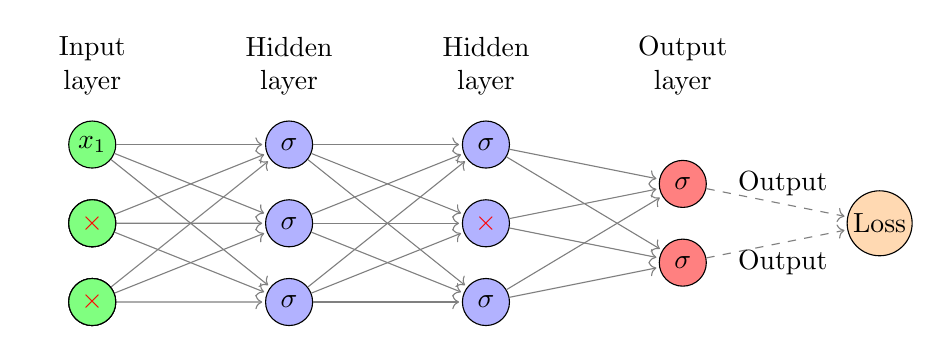
\begin{tikzpicture}[shorten >=1pt,->,draw=black!50, node distance=\layersep]
%https://tex.stackexchange.com/questions/96846/how-to-place-label-in-middle-of-line-above-and-below-with-tikz
    \tikzstyle{every pin edge}=[<-,shorten <=1pt]
    \tikzstyle{neuron}=[circle,fill=black!25,minimum size=17pt,inner sep=0pt, draw=black]
    \tikzstyle{input neuron}=[neuron, fill=green!50];
    \tikzstyle{output neuron}=[neuron, fill=red!50];
    \tikzstyle{hidden neuron}=[neuron, fill=blue!30];
    \tikzstyle{loss neuron}=[neuron, fill=orange!30];
    \tikzstyle{annot} = [text width=4em, text centered]

    % Draw the input layer nodes
    \foreach \name / \y in {1,...,3}
    % This is the same as writing \foreach \name / \y in {1/1,2/2,3/3,4/4}
        \node[input neuron] (I-\name) at (0,-\y) {$x_\y$};
        
        
    % Draw the input layer nodes
    \foreach \name / \y in {2,...,3}
    % This is the same as writing \foreach \name / \y in {1/1,2/2,3/3,4/4}
        \node[input neuron] (I-\name) at (0,-\y) {$x_\y$};
        
    % Draw the input layer nodes
    \foreach \name / \y in {2,...,3}
    % This is the same as writing \foreach \name / \y in {1/1,2/2,3/3,4/4}
        \node[input neuron] (I-\name) at (0,-\y) {\color{red}$\times$};

    % Draw the hidden layer nodes
    \foreach \name / \y in {1,...,3}
        \path[yshift=0cm]
            node[hidden neuron] (H1-\name) at (\layersep,-\y cm) {$\, \sigma\, $};

    % Draw the hidden layer nodes
    \foreach \name / \y in {1,3}
        \path[yshift=0cm]
            node[hidden neuron] (H2-\name) at (\layersep + \layersep,-\y cm) {$\, \sigma\, $};
            
            
    % Draw the hidden layer nodes
    \foreach \name / \y in {2}
        \path[yshift=0cm]
            node[hidden neuron] (H2-\name) at (\layersep + \layersep,-\y cm) {\color{red}$\, \times\, $};


    % Draw the output layer node
    \foreach \name / \y in {1,...,2}
    		\node[output neuron] (O-\y) at (\layersep + \layersep + \layersep,-\y cm-.5cm) {$\,\sigma\,$};
    		
    		
    		
    		\node[loss neuron] (L) at (\layersep +\layersep + \layersep + \layersep,-2 cm) {$\,$Loss$\,$};

    % Connect every node in the input layer with every node in the
    % hidden layer.
    \foreach \source in {1,...,3}
        \foreach \dest in {1,...,3}
            \draw (I-\source) --  (H1-\dest);

    % Connect every node in the input layer with every node in the
    % hidden layer.
    \foreach \source in {1,...,3}
        \foreach \dest in {1,...,3}
            \draw (H1-\source) --  (H2-\dest);


    % Connect every node in the hidden layer with the output layer
    \foreach \source in {1,...,3}
		\foreach \dest in {1,...,2}
        		\path (H2-\source) edge (O-\dest);
        		
		\foreach \source in {1,...,2}
        		\path[dashed] (O-\source) edge (L);

    % Annotate the layers
    \node[annot, right of=O-1,xshift=-35] {Output};
    \node[annot, right of=O-2,xshift=-35] {Output};
    \node[annot,above of=H1-1, node distance=1cm] (hl) {Hidden layer};
    \node[annot,left of=hl] {Input layer};
    \node[annot,right of=hl] (hl2) {Hidden layer};
    \node[annot,right of=hl2] {Output layer};

\end{tikzpicture}
  \end{minipage}
  \vfill
\begin{minipage}[t][0.5\textheight][t]{\textwidth}
Dropout is one of the most popular regularization modes and has been shown to be wildly successful on a range of tasks. The algorithm is very straight forward: At every training step, every node (including the input nodes but not including the output nodes) has a probability $p$ of being completely ignored for computational and training purposes. 
\end{minipage}
\end{frame}





\begin{frame}[fragile]{Dropout}
Empirical testing has show that the dropout rate $p$ should be set to
\begin{center}
\begin{table}[]
\begin{tabular}{ll}
Network Type & $p$     \\
DNN          & .1 - .5 \\
CNN          & .4 - .5   \\
RNN          & .2 - .3  
\end{tabular}
\end{table}
\end{center}
The idea behind dropout is that the network has to learn the same representation using different pathways. This forces a kind of crowd sourcing, where many ``experts'' within the network come to their own conclusion about the results and are then allowed to vote on the final outcome. Since these subnetworks will learn different features (and are easier to train) we get a better overall classifier. 
\end{frame}





\begin{frame}[fragile]{Monte Carlo and Dropout}
In 2016, Gal and Ghahramani gave additional reasons to use dropout layers. Their paper first established a mathematical justification for the use of dropout layers in terms of approximate Bayesian inference. It then proposed a method of using networks trained with dropout to yield even more accurate predictions. 

The idea is to use a dropout Monte Carlo simulation to improve accuracy after training. That, for each data point we would like prediction on, we instead make $M$ predictions with dropout enabled on the network and then average the results. The idea is to directly use the trained subnetworks to vote on the result of a new prediction. 

MC Dropout can be much more accurate (although it takes longer to run) and trains exactly the same as dropout.
\end{frame}





\begin{frame}[fragile]{Summary}
In this lecture, we've summarized the results of Geron, Chapter 11. As a starting point for DNN's, Geron provides the following helpful summary:

\begin{center}
\begin{table}[]
\begin{tabular}{ll}
Hyperparameter &  Default value \\ \hline
Kernel initializer & He initialization\\
Activation function & ELU\\
Normalization & None if shallow; Batch Norm if deep\\
Regularization & Early stopping ($+\ell_2$ reg. if needed)\\
Optimizer & Momentum optimization (or RMSProp or Nadam)\\
Learning rate schedule & 1cycle
\end{tabular}
\end{table}
\end{center}
For more information on Learning Schedules, see Geron. 
\end{frame}









\end{document}

%%%%%%%%%%%%%%%%%%%%%%%%%%%%%%%%%%
%
% |   __|___ _| |  |    \ ___ ___ _ _ _____ ___ ___| |_ 
% |   __|   | . |  |  |  | . |  _| | |     | -_|   |  _|
% |_____|_|_|___|  |____/|___|___|___|_|_|_|___|_|_|_|                                                   
%
%%%%%%%%%%%%%%%%%%%%%%%%%%%%%%%%%%



%%%%%%%%%%%%%%%%%%%%%%%%%%%%%%%%%%%%%%%%%%%
%%%%%%%%%%%%%%%%%%%%%%%%%%%%%%%%%%%%%%%%%%%
%%%%%%%%%%%%%%%%%%%%%%%%%%%%%%%%%%%%%%%%%%%



\begin{frame}[fragile]{Introduction}

\end{frame}




\begin{frame}[fragile]{Binary Classification}
  \begin{minipage}[t][0.5\textheight][t]{\textwidth}
	\centering \includegraphics[height=0.5\textheight]{.png} 
  \end{minipage}
  \vfill
\begin{minipage}[t][0.5\textheight][t]{\textwidth}

\end{minipage}
\end{frame}



\begin{frame}[fragile]{Test}
\begin{minipage}[t][0.5\textheight][t]{\textwidth}\centering
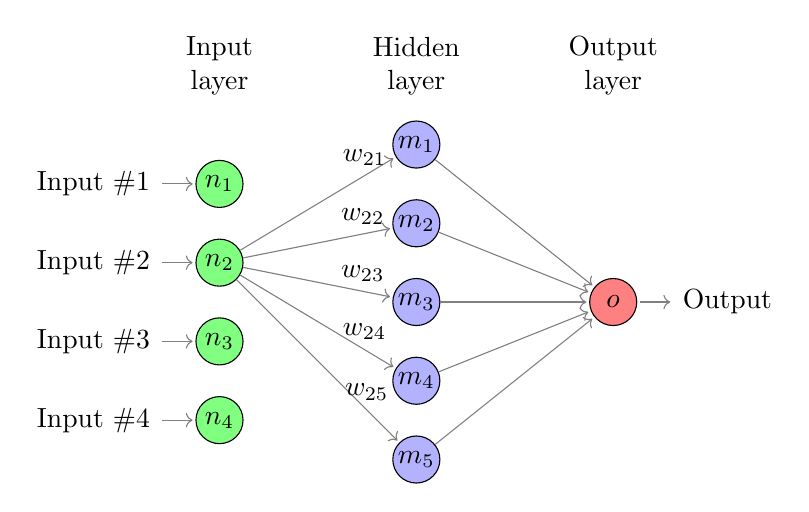
\begin{tikzpicture}[shorten >=1pt,->,draw=black!50, node distance=\layersep]
%https://tex.stackexchange.com/questions/96846/how-to-place-label-in-middle-of-line-above-and-below-with-tikz
    \tikzstyle{every pin edge}=[<-,shorten <=1pt]
    \tikzstyle{neuron}=[circle,fill=black!25,minimum size=17pt,inner sep=0pt, draw=black]
    \tikzstyle{input neuron}=[neuron, fill=green!50];
    \tikzstyle{output neuron}=[neuron, fill=red!50];
    \tikzstyle{hidden neuron}=[neuron, fill=blue!30];
    \tikzstyle{annot} = [text width=4em, text centered]

    % Draw the input layer nodes
    \foreach \name / \y in {1,...,4}
    % This is the same as writing \foreach \name / \y in {1/1,2/2,3/3,4/4}
        \node[input neuron, pin=left:Input \#\y] (I-\name) at (0,-\y) {$n_\y$};

    % Draw the hidden layer nodes
    \foreach \name / \y in {1,...,5}
        \path[yshift=0.5cm]
            node[hidden neuron] (H-\name) at (\layersep,-\y cm) {$m_\y$};

    % Draw the output layer node
    \node[output neuron,pin={[pin edge={->}]right:Output}, right of=H-3] (O) {$o$};

    % Connect every node in the input layer with every node in the
    % hidden layer.
%    \foreach \source in {1,...,4}
%        \foreach \dest in {1,...,5}
%            \draw (I-\source) -- node[below] {$w_ij$} ++ (H-\dest);


%    \foreach \source in {1,...,4}
        \foreach \dest in {1,...,5}
            \draw (I-2) -- node[above, pos=0.8] {$w_{2\dest}$} ++ (H-\dest);

    % Connect every node in the hidden layer with the output layer
    \foreach \source in {1,...,5}
        \path (H-\source) edge (O);

    % Annotate the layers
    \node[annot,above of=H-1, node distance=1cm] (hl) {Hidden layer};
    \node[annot,left of=hl] {Input layer};
    \node[annot,right of=hl] {Output layer};
\end{tikzpicture}
  \end{minipage}
  \vfill
\begin{minipage}[t][0.5\textheight][t]{\textwidth}

\end{minipage}


\end{frame}




\begin{frame}[fragile]{Point Variance of Linear Predictor}

\begin{align*}
\action<+->{ &=&&}
\\
\action<+->{  &=   && }
\end{align*}
\action<+->{The}
\end{frame}



\begin{frame}[fragile]{Correlation}
\begin{itemize}
\item[] \textbf{Serial No.} is basically uncorrelated with anything. \pause
\item[] \textbf{Admit} is highly correlated with \textbf{CGPA}, \textbf{TOEFL Score} and \textbf{GRE Score}\pause
\item[] \textbf{Research} has a lowish correlation with \textbf{Admit}, but also with everything else.  
\end{itemize}
\end{frame}











\begin{frame}[fragile]{Bias, Variance and Parameters}
  \begin{minipage}[t][0.5\textheight][t]{\textwidth}
	\centering
	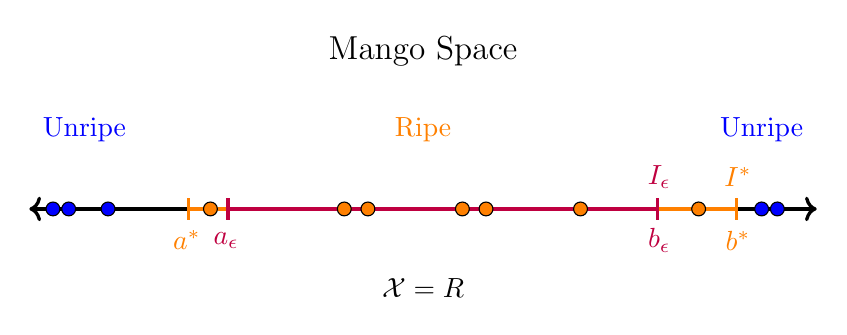
\begin{tikzpicture}
		\draw[<->,very thick] (-5,0) -- (5,0);
		\draw[color = orange, |-|,very thick] (-3,0) -- (4,0);
		\node[color=orange] at (4,.4) {$I^*$};
		\node at (0,2) {\large Mango Space} ;
		\node at (0,-1) {$\mathcal{X} = \mathbb{R}$} ;
		\node [color=blue] at (-4.3,1) {Unripe} ;
		\node [color=blue] at (4.3,1) {Unripe} ;
		\node [color=orange] at (0,1) {Ripe} ;

		\node [color=orange] at (-3,-.4) {$a^*$} ;
		\node [color=orange] at (4,-.4) {$b^*$} ;

		\draw [color=purple, |-|,very thick] (-2.5,0) -- (3,0);
		\node [color=purple] at (3,.4) {$I_\epsilon$} ;
		\node [color=purple] at (-2.5,-.4) {$a_\epsilon$} ;
		\node [color=purple] at (3,-.4) {$b_\epsilon$} ;

%		\draw [color=olive, |-|,very thick] (-3.5,0) -- (2.5,0);
%		\node [color=olive] at (3,.4) {$h_{\mathcal{T}}$} ;



		\node[circle,draw=black, fill=orange, inner sep=0pt,minimum size=5pt] at (2,0) {};
		\node[circle,draw=black, fill=orange, inner sep=0pt,minimum size=5pt] at (-1,0) {};
		\node[circle,draw=black, fill=orange, inner sep=0pt,minimum size=5pt] at (-.7,0) {};
		\node[circle,draw=black, fill=orange, inner sep=0pt,minimum size=5pt] at (.5,0) {};
		\node[circle,draw=black, fill=orange, inner sep=0pt,minimum size=5pt] at (.8,0) {};
		\node[circle,draw=black, fill=orange, inner sep=0pt,minimum size=5pt] at (-2.7,0) {};
		\node[circle,draw=black, fill=orange, inner sep=0pt,minimum size=5pt] at (3.5,0) {};

		\node[circle,draw=black, fill=blue, inner sep=0pt,minimum size=5pt] at (-4.5,0) {};
		\node[circle,draw=black, fill=blue, inner sep=0pt,minimum size=5pt] at (-4,0) {};
		\node[circle,draw=black, fill=blue, inner sep=0pt,minimum size=5pt] at (-4.7,0) {};
		\node[circle,draw=black, fill=blue, inner sep=0pt,minimum size=5pt] at (4.3,0) {};
		\node[circle,draw=black, fill=blue, inner sep=0pt,minimum size=5pt] at (4.5,0) {};
	\end{tikzpicture}
  \end{minipage}
  \vfill
  \begin{minipage}[t][0.5\textheight][t]{\textwidth}
Lets understand this visually.
$$
Err(x_0) = \sigma_\epsilon^2 + [E_\cT[\hat f(x_0)] - f(x_0)]^2 + E_\cT\big[ \hat{f}(x_0) - E_\cT[\hat{f}(x_0)] \big]^2\,.
$$\pause
Consider a data set, 
\end{minipage}
\end{frame}





























